%************************************************
\chapter{Are Humans Evolving}
%************************************************
\section{Objective}
To study the
\begin{enumerate}
	\item heritability of height in humans
	\item effect of height on Darwinian fitness
\end{enumerate}

\section{Requirements}
	\begin{enumerate}
		\item A measuring tape
		\item Weighing balance
		\item Set of humans from various parts of the country interested in performing the experiment
	\end{enumerate}

\section{Procedure}
	\begin{enumerate}
		\item The set of humans was asked to collect pedigree data for their families, where data means height of the individual (if age > 18 years), date of birth, date of marriage, weight and region.
		\item The data was then collected into a single file to preserve privacy of the people involved.
	\end{enumerate}

\section{Observations and Results}
	\begin{enumerate}
		\item 
			Heritability of Height:
			\par
			Offspring height, when plotted against the mid-parent height yields heritability. This measures the proportion of observable difference in a trait between individuals within a population that is due to genetic differences. Heritability is essentially a genetic component of variation, in the total phenotypic variation. The graph obtained is given in \autoref{human_midparent}. The heritability was found to be 0.554 which manifests that height is heritable.
			\par
			NOTE: The points seems very scattered as the graph doesn't start from zero.
		\item 
			Effect of Height on number of offspring
			\par
			I did not get a chance to react to the idea of this analysis, since Vivek had already described to me how this appeared to be rather pointless on the basis of cause, as family planning and other aspects dominate such issues and yet a co-relation exists as is manifested in \autoref{human_father} and in \autoref{human_mother}. 
			\par
			The data seems to suggest that Darwinian fitness of females are high if they're taller than average or shorter than average. However, their fitness is lower if their height is close to the average. 
			\par
			For Males, the data suggests that taller males are better in terms of Darwinian fitness.
		\item
			Distribution of month of birth of the first child
			\par
			A graph of frequency of children vs month of their birth was plotted and to it, a $2^{nd}$ degree polynomial fitted. The result obtained is shown in \autoref{human_last}. Although the graph does seem to have a curve, suggesting a `preferred' set of months, however, on performing a chi-square test for an equal probability (linear fit), it was found that the Null hypothesis can't be rejected.
	\end{enumerate}

\begin{figure}[bth]
	\begin{center}
		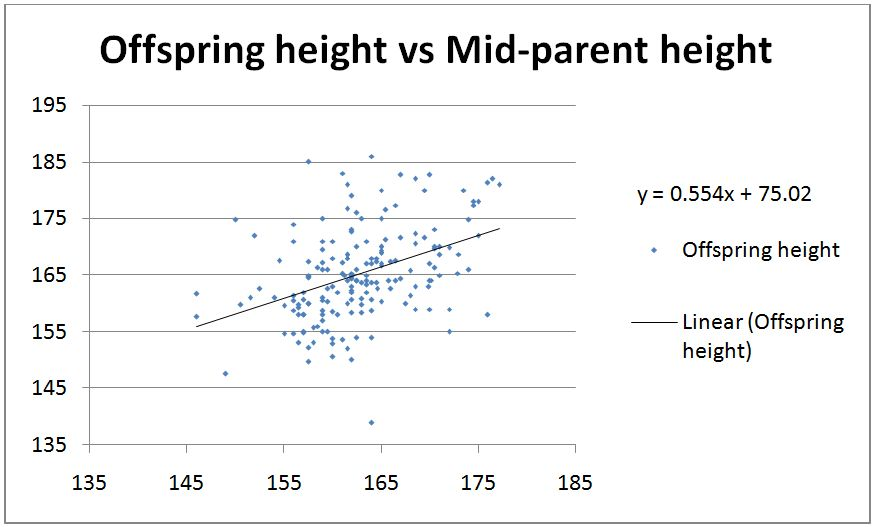
\includegraphics[width=1.1\linewidth]{gfx/Heritability_of_height}
	\end{center}
\caption[Offspring Height vs Mid-Parent Height]{Offspring Height vs Mid-Parent Height}
\label{human_midparent}
\end{figure}

\begin{figure}[bth]
	\begin{center}
		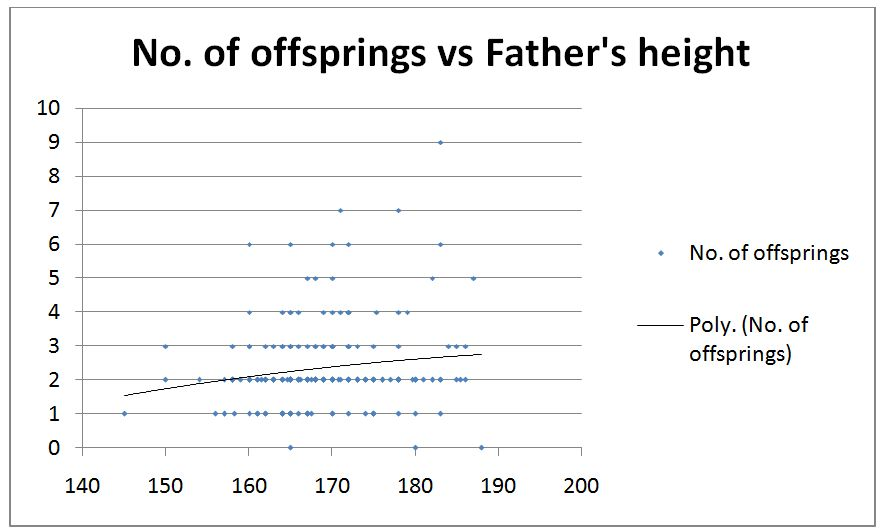
\includegraphics[width=1.1\linewidth]{gfx/Fitness_father}
	\end{center}
\caption[Number of Offspring vs Father's Height]{Number of Offspring vs Father's Height}
\label{human_father}
\end{figure}

\begin{figure}[bth]
	\begin{center}
		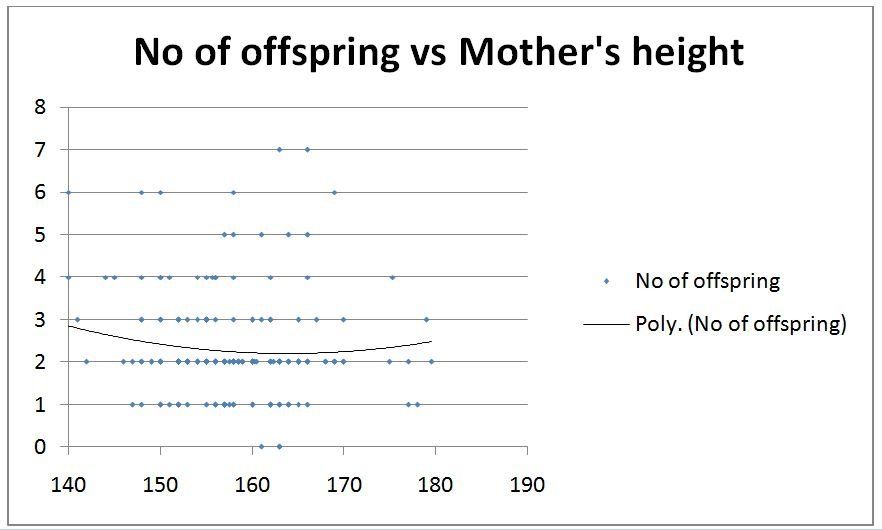
\includegraphics[width=1.1\linewidth]{gfx/Fitness_mother}
	\end{center}
\caption[Number of Offspring vs Mother's Height]{Number of Offspring vs Mother's Height}
\label{human_mother}
\end{figure}

\begin{figure}[bth]
	\begin{center}
		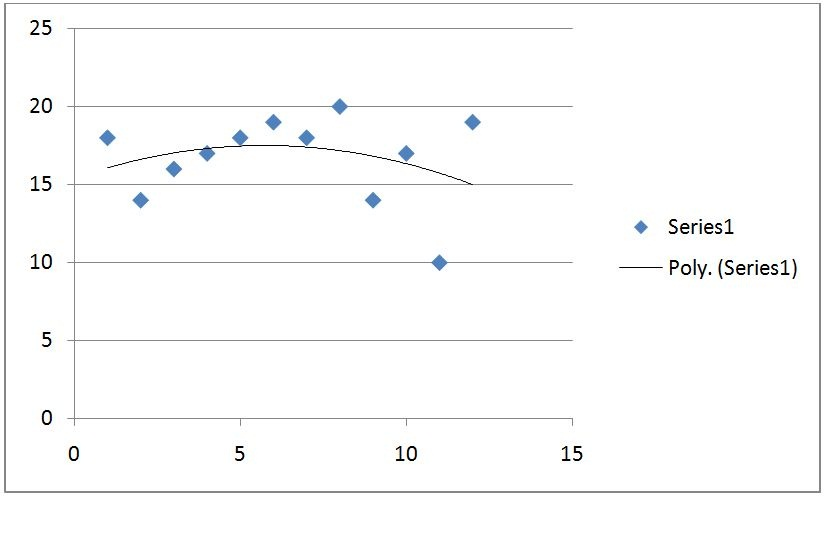
\includegraphics[width=1.1\linewidth]{gfx/Monthofbirth_first_offspring}
	\end{center}
\caption[Frequency vs Month of Birth of the first offspring]{Frequency vs Month of Birth of the first offspring}
\label{human_last}
\end{figure}

\section{Acknowledgement}
	I sincerely thank Mr. Vivek Sagar for helping me analyse this experiment since I'd missed out on the session when this was discussed. Also, the graphs were created by Vivek.
	\par
	I am grateful to our Instructor, Prof. N. G. Prasad.